\documentclass {beamer}
\usecolortheme {spruce}

\usepackage {xcolor}
\definecolor {shadow} {HTML} {423a4f}
\definecolor {system} {HTML} {debce1}
\definecolor {shade} {HTML} {554466}
\setbeamercolor {titlelike} {fg=shadow, bg=system}
\setbeamercolor {frametitle} {fg=shadow, bg=system}
\setbeamercolor {bibliography entry author} {fg=shadow}
\setbeamercolor {bibliography entry title} {fg=shadow}
\setbeamercolor {bibliography entry location} {fg=shadow}
\setbeamercolor {bibliography entry note} {fg=shadow}
\setbeamercolor {page number in head/foot} {fg=shade}

\usepackage {amsmath}
\usepackage {amssymb}
\usepackage {mathtools}
\usepackage {bbold}
\usepackage {multicol}
\usepackage {titlesec}
\usepackage {enumitem}
\usepackage {csquotes}
\usepackage {graphicx}
\usepackage {caption}
\usepackage {pgfplots}
\usepackage {tikz}
\usetikzlibrary {quantikz}

\usefonttheme [onlymath] {serif}

\DeclareMathOperator* {\argmin} {argmin}
\newcommand {\qvec}[1] {\vert #1 \rangle}
\newcommand {\qcovec}[1] {\langle #1 \vert}
\newcommand {\qeval}[1] {\langle #1 \rangle}
\newcommand {\qinner}[2] {\langle #1 \vert #2 \rangle}
\newcommand {\qouter}[2] {\qvec{#1} \qcovec{#2}}
\newcommand {\qnorm}[1] {\lVert #1 \rVert}

\defbeamertemplate {footnote} {unnumbered}	{
	\usebeamercolor [fg]{page number in head/foot}
	\usebeamerfont {page number in head/foot}
    \insertfootnotetext
}

\newcommand {\source} [1]	{
    \setbeamertemplate {footnote} [unnumbered] 
	\usebeamercolor [fg]{normal text}
    \footnotetext {\tiny #1}
}

\defbeamertemplate {footline} {centered frame number}	{
	\hspace*{\fill}
	\usebeamercolor [fg]{page number in head/foot}
	\usebeamerfont {page number in head/foot}
	\insertframenumber
	\hspace*{\fill} \vskip7pt
}
\setbeamertemplate {footline} [centered frame number]

\let \footnoterule \relax
\setbeamertemplate {navigation symbols} {}

\title	{
	Seminar: Advanced Topics in \\
	Quantum Computing \\
}
\subtitle {
	On efficient encodings for QAOA \\
	solutions to vehicle routing problems
}
\author {Eben Jowie Haezer}
\date {December 1, 2023}

\begin {document}
\maketitle


% VRP graph
\begin {frame}
\frametitle {VRP}

\centering
\pause
\begin {tikzpicture}
\filldraw[black] (0,0) circle (2pt) node[anchor=east]{depot $v_0$};
\filldraw[cyan, text=black] (3, 1) circle (2pt) node[anchor=south]{$v_j$};
\onslide <3>	{
\filldraw[cyan, text=black] (4, 2) circle (2pt) node[anchor=west]{\small[4, 6]};
}
\filldraw[cyan] (4, -0.2) circle (2pt);
\filldraw[cyan, text=black] (0.7, 0.5) circle (2pt) node[anchor=south]{$v_i$};
\onslide <3>	{
\filldraw[cyan, text=black] (1.3, 2.5) circle (2pt) node[anchor=north]{\small$d_k{=}5$};
}
\filldraw[cyan] (-1, 1.5) circle (2pt);
\filldraw (0.7, 0.5) -- node[above]{$c_{ij}$} (3, 1);
\end {tikzpicture}

\end {frame}

% VRP applications img
\begin {frame}
\frametitle {VRP}

\begin {center}
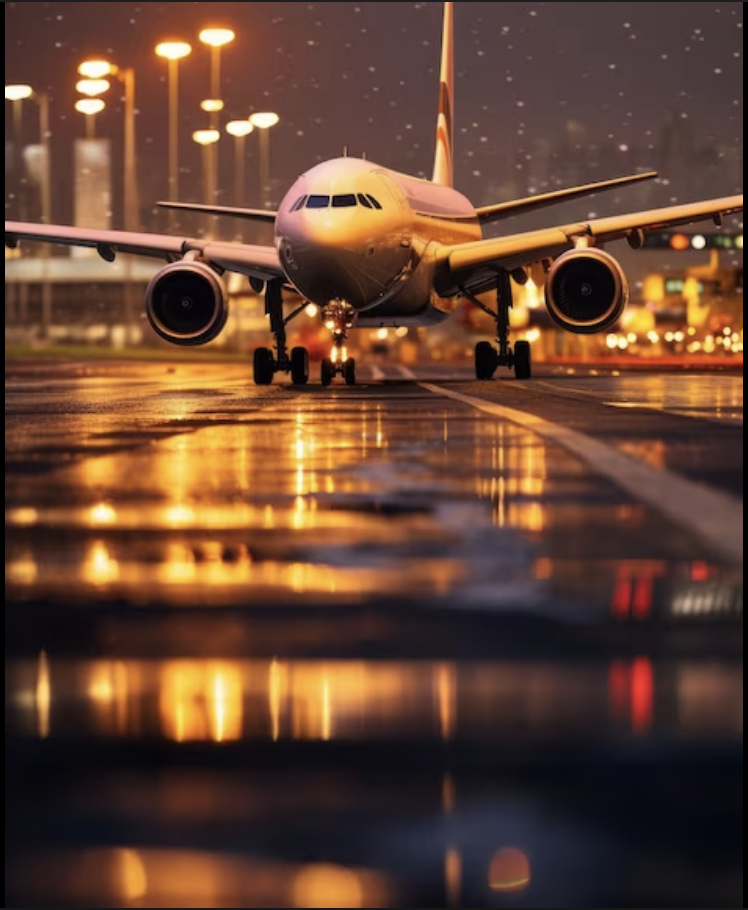
\includegraphics[width=0.45\textwidth, height=4cm] {vrp1}
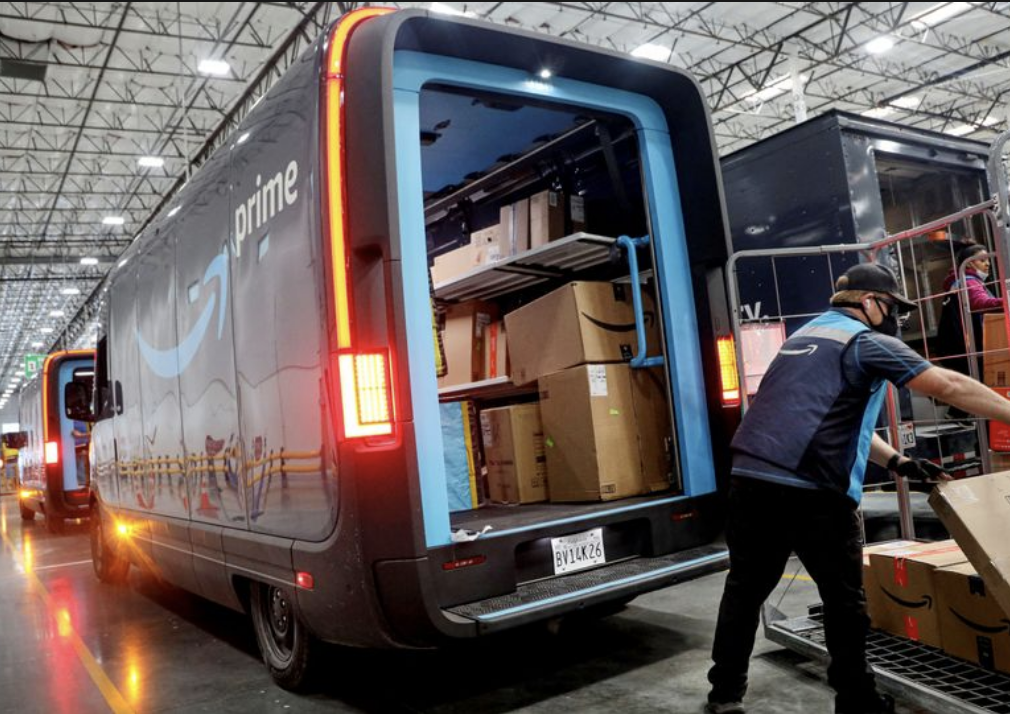
\includegraphics[width=0.45\textwidth, height=4cm] {vrp2}
\end {center}

{
\footnotesize
\url {https://www.freepik.com/free-photos-vectors/airport-night/4}
\url {https://pictures.reuters.com/}
}

\end {frame}

% adiabatic computation
\begin {frame}
\frametitle {Adiabatic computation}

\begin {displayquote}
\textit	{
A physical system remains in its instantaneous eigenstate if a given
perturbation is acting on it slowly enough and if there is a gap between the
eigenvalue and the rest of the Hamiltonian's spectrum. \cite{adiabatictheo}
}
\end {displayquote}

\pause
\begin {align*}
H(t) = \left(1 - \frac{t}{T}\right) \cdot H_0 + \frac{t}{T} \cdot H_p
\end {align*}

\end {frame}


% Lie exp prod
\begin {frame}
\frametitle {Adiabatic approximation}

\begin {align*}
\onslide<2->{\forall A, B \in \mathbb C^{m \times m}. \;}
e^{A+B} = \lim_{n \rightarrow \infty}
\big(e^{\frac{A}{n}} \cdot e^{\frac{B}{n}}\big)^n
\end {align*}

\pause

\begin {align*}
\big( \;
[A, B] = 0 \; \Longrightarrow \; e^{A+B} = e^A e^B
\; \big)
\end {align*}

\pause

\begin {align*}
\qvec{\psi(\beta, \gamma)} =
\prod_{k} e^{-i \beta_k H_x} e^{-i \gamma_k H_f}
\; \qvec{+}^{\otimes m}
\end {align*}

\source {Eq. Ref. \cite{matexp} \cite{qaoaintro}}
\end {frame}


% QAOA diagram

\begin {frame}
\frametitle {QAOA}

\begin {align*}
\qvec{\psi(\beta, \gamma)} = \prod_{k} e^{-i \beta_k H_x} e^{-i \gamma_k H_f}
\; \qvec{+}^{\otimes m}
\end {align*}

\centering
\begin {tikzpicture}
\node [scale=0.7]	{
	\begin {quantikz}
	& \gate[3]{H^{\otimes m}} & \gate[3]{e^{-i \gamma_1 H_f}}
	& \gate[3]{e^{-i \beta_1 H_x}} & \qw \ \ldots \
	& \gate[3]{e^{-i \gamma_n H_f}} & \gate[3]{e^{-i \beta_n H_x}}
	\slice{$\rvert \psi(\beta, \gamma) \rangle$}
	& \meter{} \arrow[r] &
	\\
	&&&& \qw \ \ldots \ &&& \meter{} \arrow[r] &
	\rstick{\small observe and \\ \small optimise \\ parameters}
	\\
	&&&& \qw \ \ldots \ &&& \meter{} \arrow[r] &
	\\
	&& \arrow[u] \gamma_1 & \arrow[u] \beta_1 & (\small \text{depth } n)
	& \arrow[u] \gamma_n & \arrow[u] \beta_n &&
	\end {quantikz}
};
\end {tikzpicture}
\cite{qaoaintro}

\end {frame}


% QUBO formulation
\begin {frame}
\frametitle {QUBO}

\centering
QUBO
\pause
\\
quadratic unconstrained binary optimisation
\pause
\\
\begin {align*}
\qvec{x^*} = \argmin_{\qvec{x} \in \{0, 1\}^n} \; \qcovec{x} Q \qvec{x}
\end {align*}
\pause
\\
where $Q \in \mathbb R^{n \times n}$.

\begin {align*}
f_Q(x) = \qcovec{x} Q \qvec{x} =
\sum_{i = 1}^n \sum_{j = i}^n Q_{ij} x_i x_j
\end {align*}

\source {Eq. Ref. \cite{isingnp} \cite{tutqubo}}
\end {frame}

% NP to QUBO scrshot
\begin {frame}
\frametitle {QUBO}

\begin {center}
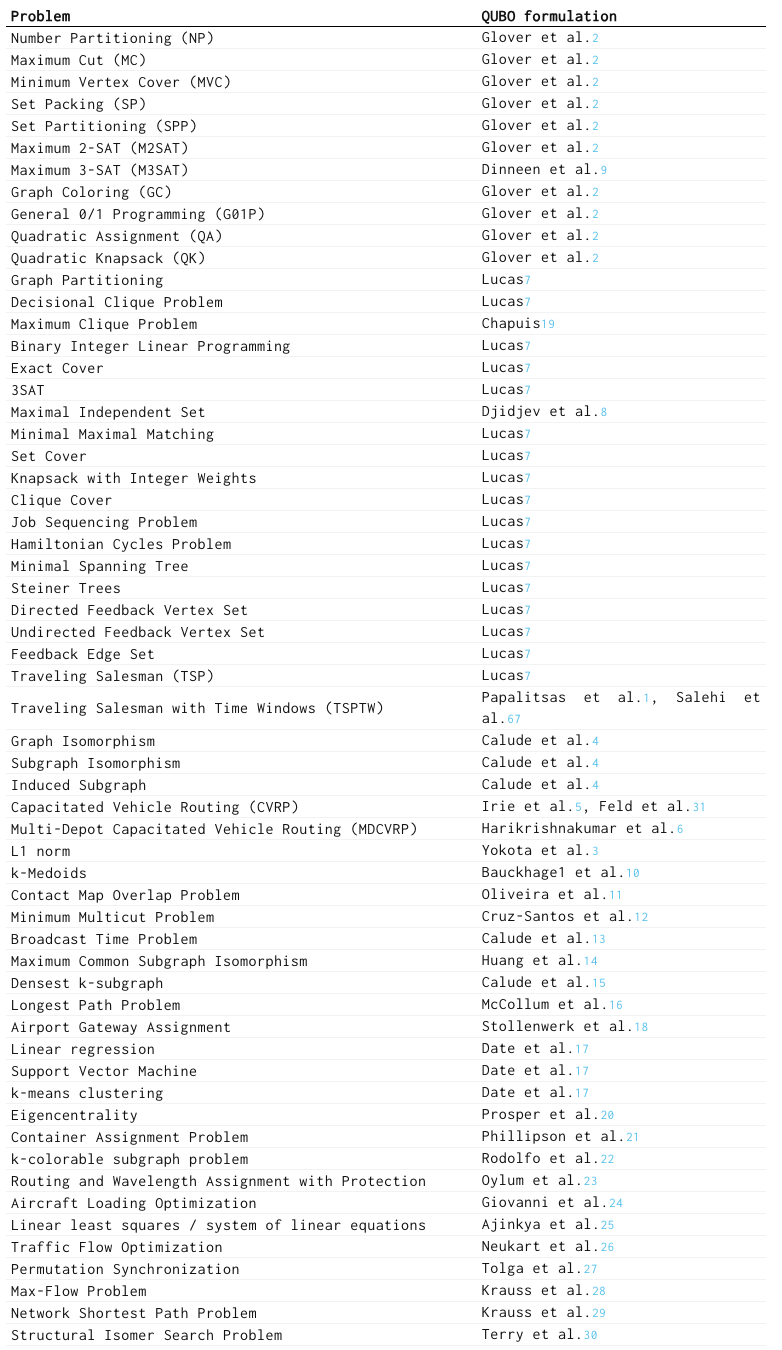
\includegraphics[width=0.4\textwidth] {qubolist1}
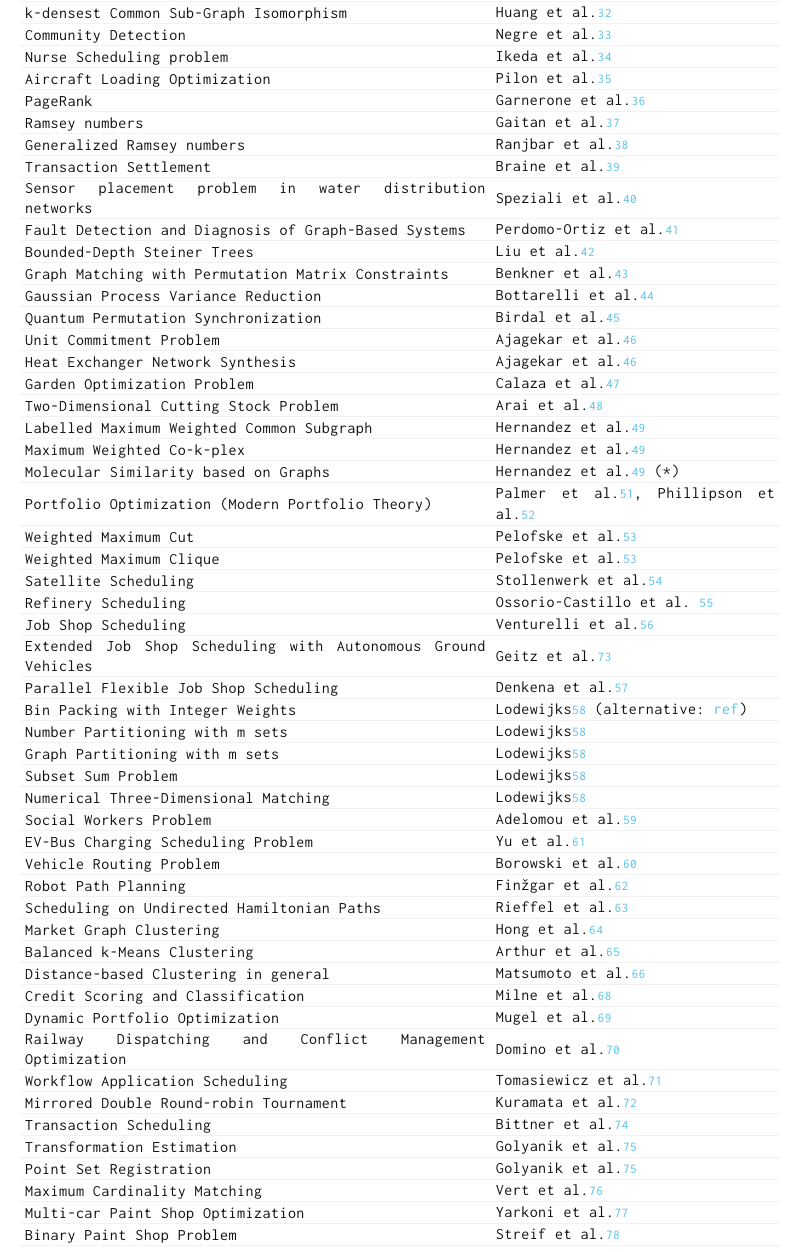
\includegraphics[width=0.4\textwidth] {qubolist2}
\cite {qubolist}
\end {center}

\end {frame}

% ising model
\begin {frame}
\frametitle {Ising model}

\begin {center}
\begin {tikzpicture}
%\draw (0, 0) circle (2pt);
%\draw (2, 0) circle (2pt);
%\draw (4, 0) circle (2pt);
%;
%\draw (1, 1) circle (2pt);
%\draw (3, 1) circle (2pt);
%\draw (5, 1) circle (2pt);
%;
%\draw (2, 2) circle (2pt);
%\draw (4, 2) circle (2pt);
%\draw (6, 2) circle (2pt);
%;
\draw[gray, dashed] (0, 0) -- (2, 0);
\draw[gray, dashed] (4, 0) -- (2, 0);
;
\draw[gray, dashed] (0, 0) -- (1, 1);
\draw[gray, dashed] (2, 0) -- (3, 1);
\draw[gray, dashed] (4, 0) -- (5, 1);
;
\draw[gray, dashed] (1, 1) -- (3, 1);
\draw[gray, dashed] (5, 1) -- (3, 1);
;
\draw[gray, dashed] (1, 1) -- (2, 2);
\draw[gray, dashed] (3, 1) -- (4, 2);
\draw[gray, dashed] (5, 1) -- (6, 2);
;
\draw[gray, dashed] (2, 2) -- (4, 2);
\draw[gray, dashed] (6, 2) -- (4, 2);
;
\draw[->] (0, -0.2) -- (0, 0.2);
\draw[->] (2, -0.2) -- (2, 0.2);
\draw[->] (4, 0.2) -- (4, -0.2);
;
\draw[->] (1, 1.2) -- (1, 0.8);
\draw[->] (3, 1.2) -- (3, 0.8);
\draw[->] (5, 0.8) -- (5, 1.2);
;
\draw[->] (2, 1.8) -- (2, 2.2);
\draw[->] (4, 1.8) -- (4, 2.2);
\draw[->] (6, 1.8) -- (6, 2.2);
;
\end {tikzpicture}
\end {center}

\pause
\begin {align*}
H = - \sum_{\qeval{i\;j}} J_{ij} \sigma_i^z \sigma_j^z
- \mu \sum_{i} h_i^z \sigma_i^z - \mu \sum_{i} h_i^x \sigma_i^x
\end {align*}

\pause
\begin {align*}
H = \sum_{z \in \{0, 1\}^n} E_z \; \qouter{z}{z}
\end {align*}

\pause
\begin {align*}
\sigma \mapsto 2x - 1, \; x \in \{0, 1\}
\end {align*}

\source {Eq. Ref. \cite{isingmodel} \cite{tutqubo}}
\end {frame}



% constraints
\begin {frame}
\frametitle {Problem Constraints}

\begin {itemize}
\pause
\item[\textbf{once}] Each customer $v_i$ in a route $r_j$ is visited exactly
	once.
\pause
\item[\textbf{step}] For each time step, each vehicle is either at a customer
	node $v_i$ or at the depot $v_0$.
\pause
\item[\textbf{cap}] All routes $\{r_i\}$ respect the maximum capacity
	$m \in \mathbb R$ of a vehicle.
\end {itemize}

\pause
\begin {align*}
H_p = H_c + p_1 H_{\text{once}} + p_2 H_{\text{step}} + p_3 H_{\text{cap}}
\end {align*}

\pause
\begin {align*}
H_{\text{once}} = \sum_i \; (1 - \sum_{r, \; t} x_{t, i}^r)^2
\end {align*}

\pause
\begin {align*}
H_{\text{step}} = \sum_{r, \; t} \; (1 - \sum_i x_{t, i}^r)^2
\end {align*}

\end {frame}

% inequality constraint
\begin {frame}
\frametitle {Constraint \textbf{cap}}

\begin {itemize}
\item[\textbf{cap}] All routes $\{r_i\}$ respect the maximum capacity
	$m \in \mathbb R$ of a vehicle.
\end {itemize}

\centering
\pause
\begin {align*}
\sum_r (m - \sum_{t, \; i} d_i x_{t, i}^r)^2 \ge 0
\end {align*}

\pause
\begin {align*}
H_{\text{cap}} = \sum_r \big( m - (\Delta + \sum_{t, \; i} d_i x_{t, i}^r) \big) ^2
\end {align*}

\pause
$d_i$: demand score for customer $v_i$

\pause
\begin {align*}
\Delta = \sum_{b = 0}^{\lceil \log_2 1+m \rceil - 1} 2^b \; a_b^r,
\; \; a_b^r \in \{0, 1\}
\end {align*}

\end {frame}

% two phase procedure
\begin {frame}
\frametitle {Two phase procedure}

\begin {align*}
H_p = H_c + p_1 H_{\text{once}} + p_2 H_{\text{step}} + p_3 H_{\text{cap}}
\end {align*}

\pause
$n_c$: number of classical binary variables

\vspace {0.3cm}

\pause
consider:
\begin {itemize}
\item[-]	number of customer nodes 
\item[-]	number of time steps required
\item[-]	routes / vehicles
\end {itemize}

\pause
\begin {align*}
n_c \in \mathcal{O}(\qnorm{V}^3)
\end {align*}

\pause
divide and conquer \cite{cvrpanneal} \cite{cvrpqaoa}
\begin {itemize}
\item[-]	clustering phase
\item[-]	routing phase
\end {itemize}

\end {frame}

% clustering
\begin {frame}
\frametitle {Clustering}

\centering
\begin {tikzpicture}
\onslide<1->	{
\filldraw[black] (0, 0) circle (2pt) node[anchor=south]{\small $v_0$};
\filldraw[black] (0, 0) circle (2pt) node[anchor=north]{\small $m{=}9$};
\filldraw[black] (3, 1) circle (2pt) node[anchor=north]{4};
\filldraw[black] (0.7, 0.5) circle (2pt) node[anchor=north]{1};
\filldraw[black] (-1, 2) circle (2pt) node[anchor=north]{2};
\filldraw[black] (3.5, 2.2) circle (2pt) node[anchor=north]{2};
\filldraw[black] (1.3, 1.9) circle (2pt) node[anchor=north]{3};
\filldraw[black] (4.1, 1.2) circle (2pt) node[anchor=north]{3};
\filldraw[black] (2.4, 0.1) circle (2pt) node[anchor=north]{2};
}
\onslide<2->	{
\filldraw[red] (3, 1) circle (2pt) node[anchor=north]{4};
\filldraw[blue] (0.7, 0.5) circle (2pt) node[anchor=north]{1};
\filldraw[blue] (-1, 2) circle (2pt) node[anchor=north]{2};
\filldraw[blue] (3.5, 2.2) circle (2pt) node[anchor=north]{2};
\filldraw[blue] (1.3, 1.9) circle (2pt) node[anchor=north]{3};
\filldraw[red] (4.1, 1.2) circle (2pt) node[anchor=north]{3};
\filldraw[red] (2.4, 0.1) circle (2pt) node[anchor=north]{2};
}
\end {tikzpicture}

\onslide<3->{subject to constraints:}
\onslide<4->{\textbf{once}, \textbf{cap}}
\\
\vspace {0.3cm}
\onslide<5->{additional constraint: \textbf{cluster}}
\\
\onslide<6->	{
	\small \textit{The cumulative edge cost $c_{ij}$ between all pairs of nodes \\
	$(i,j)$ within a cluster should be minimal.}
}
\onslide<7>	{
\begin {align*}
H_{\text{cluster}} = \sum_r \sum_{i, \; j} c_{ij} \; x_i^r \; x_j^r
\end {align*}
where $x_i^r = \sum_t x_{i, t}^k$
}
\end {frame}

% routing
\begin {frame}
\frametitle {Routing}

\centering
\begin {tikzpicture}
\onslide<2->	{
\draw[magenta, style=dashed] (0, 0) -- (3, 1) -- (4.1, 1.2) -- (2.4, 0.1)
-- (0, 0);
\draw[cyan, style=dashed] (0, 0) -- (-1, 2) -- (1.3, 1.9) -- (3.5, 2.2)
-- (0.7, 0.5) -- (0, 0);
}

\filldraw[black] (0, 0) circle (2pt) node[anchor=south]{\small $v_0$};
\filldraw[black] (0, 0) circle (2pt) node[anchor=north]{\small $m{=}9$};
\filldraw[red] (3, 1) circle (2pt) node[anchor=north]{4};
\filldraw[blue] (0.7, 0.5) circle (2pt) node[anchor=north]{1};
\filldraw[blue] (-1, 2) circle (2pt) node[anchor=north]{2};
\filldraw[blue] (3.5, 2.2) circle (2pt) node[anchor=north]{2};
\filldraw[blue] (1.3, 1.9) circle (2pt) node[anchor=north]{3};
\filldraw[red] (4.1, 1.2) circle (2pt) node[anchor=north]{3};
\filldraw[red] (2.4, 0.1) circle (2pt) node[anchor=north]{2};
\end {tikzpicture}

\onslide<3->	{
	subject to constraints: \textbf{once}, \textbf{step}, edge costs
}

\onslide<4>	{
\begin {align*}
H_{\text{tsp}} = q_1 H_{\text{once}} + q_2 H_{\text{step}} + q_3 H_c
\end {align*}
}

\end {frame}


% complete encoding
\begin {frame}
\frametitle {Complete encoding}

\centering
\begin {tikzpicture}
\node [scale=1.0]	{
	\begin {quantikz}
	& \qw & \ldots \ &[1cm] \qw \rstick[3]{\ket{\psi}}
	\\
	& \qw & \ldots \ &[1cm] \qw
	\\
	& \qw & \ldots \ &[1cm] \qw
	\end {quantikz}
};
\end {tikzpicture}

\pause
\begin {align*}
\qvec{\psi} = \sum_{z \in \{0, 1\}^n} \beta_z \; \qvec{z}
\end {align*}

\onslide<3->{$\qvec{z}$ corresponds to}
\\
\begin {tikzpicture}
\onslide<3->	{
	\filldraw[black] (0, 0) circle (2pt) node[anchor=east]{depot $v_0$};
	\filldraw (3, 1) circle (2pt);
	\filldraw (4, 2) circle (2pt);
	\filldraw (4, -0.2) circle (2pt);
	\filldraw (0.7, 0.5) circle (2pt);
}

\onslide<4>	{
	\draw[-{Stealth[magenta]}, thick, text=magenta] (0, 0) -- node[above]{1} (0.7, 0.5);
	\draw[-{Stealth[magenta]}, thick, text=magenta] (0.7, 0.5) -- node[above]{2} (3, 1);
	\draw[-{Stealth[magenta]}, thick, text=magenta] (3, 1) -- node[above]{3} (4, 2);
	\draw[-{Stealth[magenta]}, thick, text=magenta] (4, 2) -- node[right]{4} (4, -0.2);
	\draw[-{Stealth[magenta]}, thick, text=magenta] (4, -0.2) -- node[below]{5} (0, 0);
}
\end {tikzpicture}

\end {frame}

% minimal encoding intro
\begin {frame}
\frametitle {Minimal encoding}

\pause
\centering
\begin {tikzpicture}
\node [scale=1.0]	{
	\begin {quantikz}
	& \qw & \ldots \ &[1cm] \qw \rstick[3]{\ket{\phi} register}
	\\
	& \qw & \ldots \ &[1cm] \qw
	\\
	& \qw & \ldots \ &[1cm] \qw
	\\
	& \qw & \ldots \ &[1cm] \qw \rstick{\ket{z} auxiliary}
	\end {quantikz}
};
\end {tikzpicture}

\pause
register width $n_r$, aux width $n_a$, $n_q = n_r + n_a$

\pause
\begin {align*}
\qvec{\psi(\theta)} = \sum_{i=1}^{n_c} \beta_k
(a_i \qvec{0} + b_i \qvec{1}) \; \qvec{\phi_i}
\end {align*}

\pause
$\qvec{\phi_i}$ corresponds to a single classical variable $x_{i, t}^r$.

\pause
\begin {align*}
n_q = 1 + \log_2 n_c
\end {align*}

\source {Eq. Ref. \cite{effbinopt}}
\end {frame}

% minimal encoding example
\begin {frame}
\frametitle {Example}

let $n_c = 4$, $n_r = 2$. \\

\pause
\begin {align*}
x^* = (1, 1, 1, 0)^\dag
\end {align*}

\begin {align*}
\qvec{\psi^*} = \onslide<4>{\frac{1}{2}}\onslide<3->{(\qvec{1}\qvec{00} + \qvec{1}\qvec{01}
+ \qvec{1}\qvec{10} + \qvec{0}\qvec{11})}
\end {align*}

\end {frame}

% minimal encoding probability calculation
\begin {frame}
\frametitle {Solution probability}

\begin {align*}
\qvec{\psi(\theta)} = \sum_{i=1}^{n_c} \beta_k
(a_i \qvec{0} + b_i \qvec{1}) \; \qvec{\phi_i}
\end {align*}

\pause
Born rule: $\Pr (x_i = 1) = \qnorm{\qinner{1}{z_i}}^2 = \qnorm{b_i}^2$

\pause
\begin {align*}
\Pr x = \prod_{i=1}^{n_c} \Pr x_i = \prod_{i=1}^{n_c} \qnorm{b_i}^2
\end {align*}

\end {frame}

% tradeoffs
\begin {frame}
\frametitle {Tradeoffs}

\pause
\begin {align*}
\Delta x \Delta p \ge \frac{\hbar}{2}
\end {align*}

\pause
\begin {align*}
\Pr x = \prod_{i=1}^{n_c} \Pr x_i = \prod_{i=1}^{n_c} \qnorm{b_i}^2
\end {align*}

\pause
\begin {align*}
\mathrm E \; x_i &= \qnorm{b_i}^2 \\
\onslide<3->	{
	\mathrm E \; x_i x_j &= \qnorm{b_i}^2 \qnorm{b_j}^2 \\
}
\onslide<4->	{
\mathrm{cov} (x_i, x_j) &= \mathrm E \; x_i x_j
- \mathrm E \; x_i \; \mathrm E \; x_j \\
}
\onslide<5>	{
&= 0
}
\end {align*}

\end {frame}


\begin {frame}
\frametitle {Tradeoffs}

\begin {center}
\begin {tikzpicture}
\filldraw[black] (0, 0) circle (2pt) node[anchor=east]{depot $v_0$};
\filldraw[cyan] (5, 0.5) circle (2pt);
\filldraw[cyan] (5.6, 0.3) circle (2pt);
\draw (1, 1.2) circle (2pt);
\draw (-0.6, 0.7) circle (2pt);
\draw (0.2, 0.8) circle (2pt);

\onslide<2->	{
	\filldraw[cyan, text=black] (5.6, 0.3) circle (2pt) node[anchor=west]{\small $x_{i, t}^r$};
}
\onslide<3->	{
	\filldraw[cyan, text=black] (5, 0.5) circle (2pt) node[anchor=south]{\small $x_{j, t+1}^r$};
}
\end {tikzpicture}
\end {center}

\begin {align*}
\onslide<4->	{
	\qvec{\psi(\theta)} = \sum_{i=1}^{n_c} \beta_k
	(a_i \qvec{0} + b_i \qvec{1}) \; \qvec{\phi_i}
}
\end {align*}

\onslide<5>	{
example:
\begin {align*}
	\qvec{\psi^*} = \frac{1}{2}(\qvec{1}\qvec{00} + \qvec{1}\qvec{01}
	+ \qvec{1}\qvec{10} + \qvec{0}\qvec{11})
\end {align*}
}

\end {frame}


% results
\begin {frame}
\frametitle {Experimental results}

\begin {center}
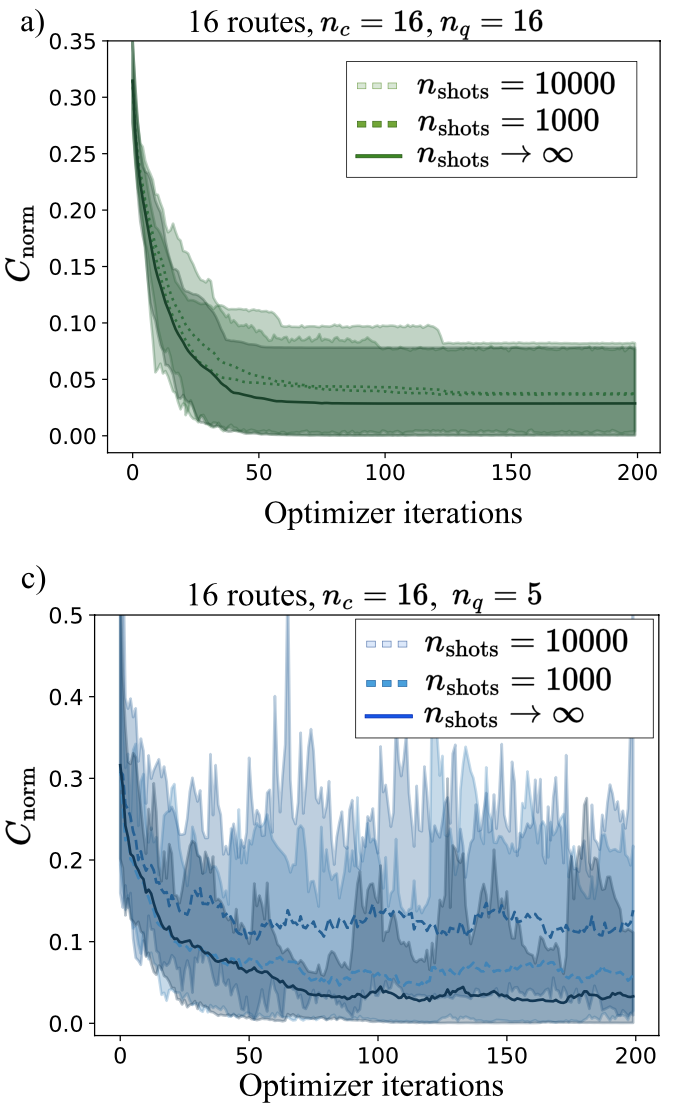
\includegraphics[width=0.28\textwidth] {2fig}
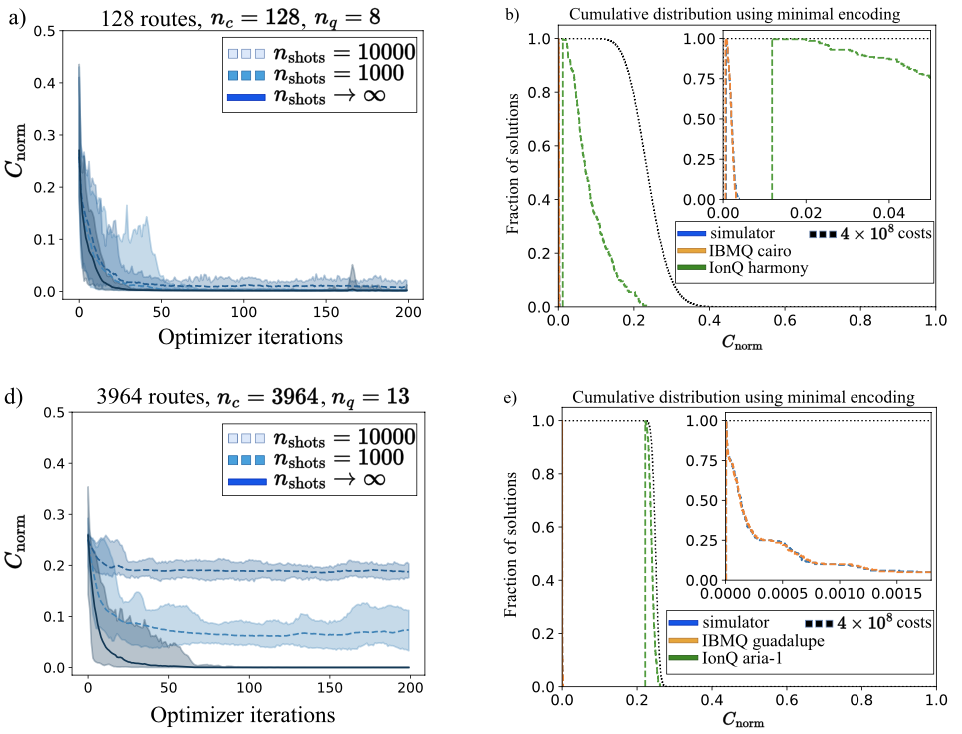
\includegraphics[width=0.6\textwidth] {4fig}
\cite{effvrp}
\end {center}

\end {frame}

% closing
\begin {frame}
\centering
Thank you for your attention.

\vfill
\url {github.com/ge42faz/qsem-23w}
\end {frame}

% backup slide: empty for notes
\begin {frame}
\frametitle {Backup slides}
\end {frame}

% backup slide: adiabatic evolution
\begin {frame}
\frametitle {Backup slides}
\framesubtitle {Adiabatic computation}

\centering
\begin {tikzpicture} [scale=1.5]
\filldraw[gray] (-1.1, 0) rectangle node[anchor=east, style={scale=0.5}]{$V \rightarrow \infty$} (-1, 1);
\node[circle, style={scale=0.5}] at (0, -0.2) {$V = 0$};
\filldraw[gray] (1, 0) rectangle node[anchor=west, style={scale=0.5}]{$V \rightarrow \infty$} (1.1, 1);

\draw[->, thick] (0, 0) -- (0, 1);
\node[circle, style={scale=0.5}] at (0, 1.2) {$E$};
\draw[<->, thick] (-1.4, 0) -- (1.4, 0);
\node[circle, style={scale=0.5}] at (1.5, 0) {$x$};
\end {tikzpicture}

\begin {align*}
i \hbar \; \frac{\partial}{\partial t} \psi(x, t) = 
\frac{- \hbar^2}{2m} \; \frac{\partial}{\partial x^2} \psi(x, t) \; + \; V(x) \; \psi(x, t)
\end {align*}

\vspace{0.3cm}
$\psi(x, t) = e^{-i \omega t} (A \sin kx + B \sin kx)$ for $x$ within the box.
\end {frame}

\begin {frame}
\frametitle {Backup slides}
\framesubtitle {Adiabatic computation}

\begin {columns}[T]
\begin {column} {0.45\textwidth}

\begin {tikzpicture}
\begin {axis} [
	width=0.8\textwidth, height=0.4\textwidth, grid=none, ticks=none,
	axis x line=bottom, axis y line=left,
	xlabel=$x$, ylabel=$\psi^2$, xmax=3.4, ymax=1.3,
	every axis x label/.style={
		at={(ticklabel* cs:1.01)},
		anchor=west,
		font=\tiny
	},
	every axis y label/.style={
		at={(ticklabel* cs:1.01)},
		anchor=south,
		font=\tiny
	},
]
\addplot [smooth, thick, domain=-pi:pi, samples=200] {cos(0.5*deg(x))*cos(0.5*deg(x))};
\end {axis}
\end {tikzpicture}

\begin {tikzpicture}
\begin {axis} [
	width=0.8\textwidth, height=0.4\textwidth, grid=none, ticks=none,
	axis x line=bottom, axis y line=left,
	xlabel=$x$, ylabel=$\psi^2$, xmax=3.4, ymax=1.3,
	every axis x label/.style={
		at={(ticklabel* cs:1.01)},
		anchor=west,
		font=\tiny
	},
	every axis y label/.style={
		at={(ticklabel* cs:1.01)},
		anchor=south,
		font=\tiny
	},
]
\addplot [smooth, thick, domain=-pi:pi, samples=200] {sin(deg(x))*sin(deg(x))};
\end {axis}
\end {tikzpicture}

\begin {tikzpicture}
\begin {axis} [
	width=0.8\textwidth, height=0.4\textwidth, grid=none, ticks=none,
	axis x line=bottom, axis y line=left,
	xlabel=$x$, ylabel=$\psi^2$, xmax=3.4, ymax=1.3,
	every axis x label/.style={
		at={(ticklabel* cs:1.01)},
		anchor=west,
		font=\tiny
	},
	every axis y label/.style={
		at={(ticklabel* cs:1.01)},
		anchor=south,
		font=\tiny
	},
]
\addplot [smooth, thick, domain=-pi:pi, samples=200] {cos(1.5*deg(x))*cos(1.5*deg(x))};
\end {axis}
\end {tikzpicture}

\begin {tikzpicture}
\begin {axis} [
	width=0.8\textwidth, height=0.4\textwidth, grid=none, ticks=none,
	axis x line=bottom, axis y line=left,
	xlabel=$x$, ylabel=$\psi^2$, xmax=3.4, ymax=1.3,
	every axis x label/.style={
		at={(ticklabel* cs:1.01)},
		anchor=west,
		font=\tiny
	},
	every axis y label/.style={
		at={(ticklabel* cs:1.01)},
		anchor=south,
		font=\tiny
	},
]
\addplot [smooth, thick, domain=-pi:pi, samples=200] {sin(2*deg(x))*sin(2*deg(x))};
\end {axis}
\end {tikzpicture}

\vspace {0.5cm}
$H \qvec{\psi} = E \qvec{\psi}$

\vspace {0.3cm}

$E_k = \hbar \omega_k = \frac{n^2 \pi^2}{L^2} \frac{\hbar^2}{2m}$

\end {column}

\begin {column} {0.45\textwidth}

\begin {tikzpicture}
\begin {axis} [
	width=0.75\textwidth, height=0.4\textwidth, grid=none, ticks=none,
	axis x line=bottom, axis y line=left,
	xlabel=$x$, ylabel=$\psi^2$, xmax=3.4, ymax=1.3,
	every axis x label/.style={
		at={(ticklabel* cs:1.01)},
		anchor=west,
		font=\tiny
	},
	every axis y label/.style={
		at={(ticklabel* cs:1.01)},
		anchor=south,
		font=\tiny
	},
]
\addplot [smooth, thick, domain=-pi:pi, samples=200] {cos(0.5*deg(x))*cos(0.5*deg(x))};
\end {axis}
\end {tikzpicture}

\begin {tikzpicture}
\begin {axis} [
	width=\textwidth, height=0.4\textwidth, grid=none, ticks=none,
	axis x line=bottom, axis y line=left,
	xlabel=$x$, ylabel=$\psi^2$, xmax=6.5, ymax=1.3,
	every axis x label/.style={
		at={(ticklabel* cs:1.01)},
		anchor=west,
		font=\tiny
	},
	every axis y label/.style={
		at={(ticklabel* cs:1.01)},
		anchor=south,
		font=\tiny
	},
]
\addplot [smooth, thick, domain=-2*pi:2*pi, samples=200] {cos(0.25*deg(x))*cos(0.25*deg(x))};
\end {axis}
\end {tikzpicture}

\begin {tikzpicture}
\begin {axis} [
	width=\textwidth, height=0.4\textwidth, grid=none, ticks=none,
	axis x line=bottom, axis y line=left,
	xlabel=$x$, ylabel=$\psi^2$, xmax=6.5, ymax=1.3,
	every axis x label/.style={
		at={(ticklabel* cs:1.01)},
		anchor=west,
		font=\tiny
	},
	every axis y label/.style={
		at={(ticklabel* cs:1.01)},
		anchor=south,
		font=\tiny
	},
]
\addplot [smooth, thick, domain=-pi:pi, samples=200] {cos(0.5*deg(x))*cos(0.5*deg(x))};
\end {axis}
\end {tikzpicture}

\vspace{0.5cm}
$H(t) = \left(1 - \frac{t}{T}\right) \cdot H_0 + \frac{t}{T} \cdot H_p$

\vspace{0.3cm}
$0 \leq t \leq 1$, $T \in \mathcal{O}(\frac{1}{g^2})$

\vspace{0.3cm}
$[H_0, H_p] \neq 0$

\end {column}

\end {columns}
\end {frame}

% backup slide: Ising model
\begin {frame}
\frametitle {Backup slides}
\framesubtitle {Ising model}

\centering
\begin {align*}
\mathbf{B} = \frac{\mu_0}{4\pi} \; \big(\frac{3\mathbf{r(m \cdot r)}}{r^5}
- \frac{\mathbf{m}}{r^3}\big)
\end {align*}

\begin {align*}
H = - \sum_{\qeval{i\;j}} J_{ij} \sigma_i \sigma_j + \mu \sum_{i} h_i \sigma_i
\end {align*}

$\mu = \frac{-e}{2m_e} L$

\vspace {0.3cm}
$J_{ij} > 0$ ferromagnetic, $J_{ij} < 0$ antiferromagnetic.

\end {frame}

% backup slide: cost function
\begin {frame}
\frametitle {Backup slides}
\framesubtitle {Cost function}
\centering

\begin {align*}
C_{\text{cpl}}(\theta) = \qeval{H} = \qcovec{\psi(\theta)} H \qvec{\psi(\theta)}
\end {align*}

\begin {align*}
C_{\text{min}}(\theta)
&= \sum_{i \neq j}^{n_c} Q_{ij} \qnorm{b_i}^2 \qnorm{b_j}^2
+ \sum_{i=1}^{n_c} Q_{ii} \qnorm{b_i}^2 \\
&= \sum_{i \neq j}^{n_c} Q_{ij}
\frac{\qeval{P_i^1}}{\qeval{P_i}} \frac{\qeval{P_j^1}}{\qeval{P_j}}
+ \sum_{i=1}^{n_c} Q_{ii} \frac {\qeval{P_i^1}} {P_i}
\end {align*}
expressed as projectors $P_i = \qouter{\phi_i}{\phi_i}$ and
$P_i^1 = \qouter{1}{1} \otimes P_i$.

\begin {align*}
\overline{C} = \frac{C(\theta) - C^*}{\Delta C}
\end {align*}

\end {frame}


% backup slide: qaoa stepwise
% fr0
\begin {frame}
\frametitle {Backup slides}
\framesubtitle {QAOA}

\begin {align*}
\qvec{\psi(\beta, \gamma)} =
\invisible{\prod_{k} e^{-i \beta_k H_x} e^{-i \gamma_k H_f}
\; \qvec{+}^{\otimes m}}
\end {align*}

\centering
\begin {tikzpicture}
\node [scale=0.7]	{
	\begin {quantikz}
	&
	\\
	&
	\\
	&
	\end {quantikz}
};
\end {tikzpicture}
\end {frame}
% fr1
\begin {frame}
\frametitle {Backup slides}
\framesubtitle {QAOA}

\begin {align*}
\qvec{\psi(\beta, \gamma)} =
\invisible{\prod_{k} e^{-i \beta_k H_x} e^{-i \gamma_k H_f}}
\; \qvec{+}^{\otimes m}
\end {align*}

\centering
\begin {tikzpicture}
\node [scale=0.7]	{
	\begin {quantikz}
	& \gate[3]{H^{\otimes m}} 
	\\
	&
	\\
	&
	\end {quantikz}
};
\end {tikzpicture}
\end {frame}

% fr2
\begin {frame}
\frametitle {Backup slides}
\framesubtitle {QAOA}

\begin {align*}
\qvec{\psi(\beta, \gamma)} =
\invisible{\prod_{k} e^{-i \beta_k H_x}} e^{-i \gamma_k H_f}
\; \qvec{+}^{\otimes m}
\end {align*}

\centering
\begin {tikzpicture}
\node [scale=0.7]	{
	\begin {quantikz}
	& \gate[3]{H^{\otimes m}} & \gate[3]{e^{-i \gamma_1 H_f}} 
	\\
	&&
	\\
	&&
	\end {quantikz}
};
\end {tikzpicture}
\end {frame}

% fr3
\begin {frame}
\frametitle {Backup slides}
\framesubtitle {QAOA}

\begin {align*}
\qvec{\psi(\beta, \gamma)} =
\invisible{\prod_{k}} e^{-i \beta_k H_x} e^{-i \gamma_k H_f}
\; \qvec{+}^{\otimes m}
\end {align*}

\centering
\begin {tikzpicture}
\node [scale=0.7]	{
	\begin {quantikz}
	& \gate[3]{H^{\otimes m}} & \gate[3]{e^{-i \gamma_1 H_f}} 
	& \gate[3]{e^{-i \beta_1 H_x}} &
	\\
	&&&
	\\
	&&&
	\end {quantikz}
};
\end {tikzpicture}
\end {frame}

% fr4
\begin {frame}
\frametitle {Backup slides}
\framesubtitle {QAOA}

\begin {align*}
\qvec{\psi(\beta, \gamma)} =
\prod_{k} e^{-i \beta_k H_x} e^{-i \gamma_k H_f}
\; \qvec{+}^{\otimes m}
\end {align*}

\centering
\begin {tikzpicture}
\node [scale=0.7]	{
	\begin {quantikz}
	& \gate[3]{H^{\otimes m}} & \gate[3]{e^{-i \gamma_1 H_f}}
	& \gate[3]{e^{-i \beta_1 H_x}} & \qw \ \ldots \
	& \gate[3]{e^{-i \gamma_n H_f}} & \gate[3]{e^{-i \beta_n H_x}}
	\\
	&&&& \qw \ \ldots \ &&&
	\\
	&&&& \qw \ \ldots \ &&&
	\\
	&&&& (\small \text{depth } n) &&&
	\end {quantikz}
};
\end {tikzpicture}
\end {frame}

% fr5
\begin {frame}
\frametitle {Backup slides}
\framesubtitle {QAOA}

\begin {align*}
\qvec{\psi(\beta, \gamma)} = \prod_{k} e^{-i \beta_k H_x} e^{-i \gamma_k H_f}
\; \qvec{+}^{\otimes m}
\end {align*}

\centering
\begin {tikzpicture}
\node [scale=0.7]	{
	\begin {quantikz}
	& \gate[3]{H^{\otimes m}} & \gate[3]{e^{-i \gamma_1 H_f}}
	& \gate[3]{e^{-i \beta_1 H_x}} & \qw \ \ldots \
	& \gate[3]{e^{-i \gamma_n H_f}} & \gate[3]{e^{-i \beta_n H_x}}
	\slice{$\rvert \psi(\beta, \gamma) \rangle$}
	& \meter{} \arrow[r] &
	\\
	&&&& \qw \ \ldots \ &&& \meter{} \arrow[r] &
	\rstick{\small observe and \\ \small optimise \\ parameters}
	\\
	&&&& \qw \ \ldots \ &&& \meter{} \arrow[r] &
	\\
	&& \arrow[u] \gamma_1 & \arrow[u] \beta_1 & (\small \text{depth } n)
	& \arrow[u] \gamma_n & \arrow[u] \beta_n &&
	\end {quantikz}
};
\end {tikzpicture}
\end {frame}


\bibliographystyle {IEEEtran}
\begin {frame} [allowframebreaks]
\frametitle {References}
\bibliography {slides}
\end {frame}

\end {document}

